\section{my\-Dialog::Save\-FITSFile\-Dialog Class Reference}
\label{classmyDialog_1_1SaveFITSFileDialog}\index{myDialog::SaveFITSFileDialog@{myDialog::SaveFITSFileDialog}}
Inheritance diagram for my\-Dialog::Save\-FITSFile\-Dialog::\begin{figure}[H]
\begin{center}
\leavevmode
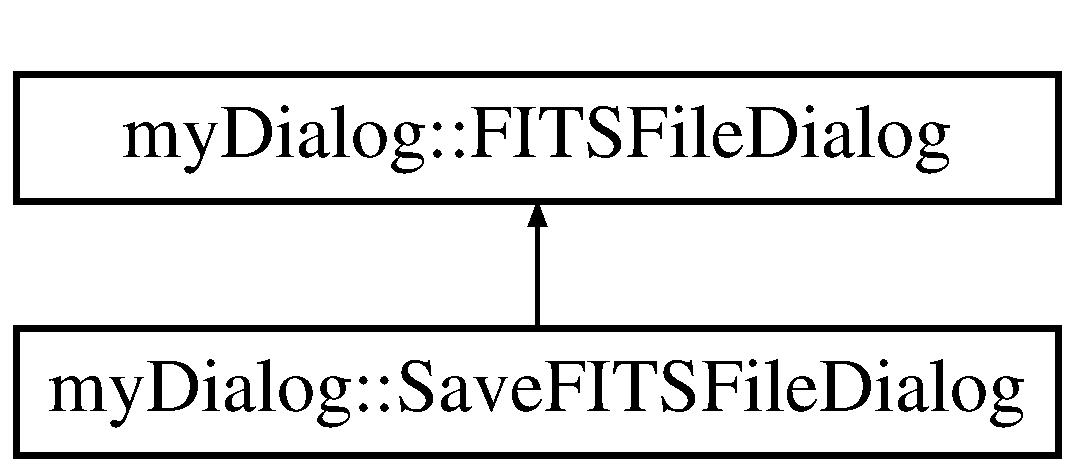
\includegraphics[height=2cm]{classmyDialog_1_1SaveFITSFileDialog}
\end{center}
\end{figure}
\subsection*{Public Member Functions}
\begin{CompactItemize}
\item 
def \textbf{ok\_\-command}\label{classmyDialog_1_1SaveFITSFileDialog_194944e127e2a406375d9fb4fe692736}

\item 
def \textbf{set\_\-selection}\label{classmyDialog_1_1SaveFITSFileDialog_9769e3a5c6ac4096d9d6f418c215bfa8}

\end{CompactItemize}
\subsection*{Static Public Attributes}
\begin{CompactItemize}
\item 
string \textbf{title} = \char`\"{}Select File\char`\"{}\label{classmyDialog_1_1SaveFITSFileDialog_9c6b6a9c577c977075ba921d77a90d45}

\end{CompactItemize}


\subsection{Detailed Description}


\footnotesize\begin{verbatim}File selection dialog which checks that the file may be created.\end{verbatim}
\normalsize
 



The documentation for this class was generated from the following file:\begin{CompactItemize}
\item 
old/PANICtool-1.0/my\-Dialog.py\end{CompactItemize}
